\documentclass[journal]{IEEEtran}
\IEEEoverridecommandlockouts
\usepackage{graphics}
\usepackage{rotating}
\usepackage{epsfig}
\usepackage{amsmath}
\usepackage{amssymb}
\usepackage[spanish]{babel}
\usepackage{cite}
\usepackage{hyperref}
\usepackage{float}
\usepackage{csvsimple}
\usepackage{atbegshi} % erase first blank page
\AtBeginDocument{\AtBeginShipoutNext{\AtBeginShipoutDiscard}}

\title{\LARGE \bf Ruteo de entrega de productos para una empresa de e-commerce}

\author{Verónica Victoria García De la Fuente, Emily Rebeca Méndez Cruz, \\Carolina Longoria Lozano, Juan Pablo Echeagaray González \\
Optimización determinista \\
MA2001B.200 \\
Dr. Fernando Elizalde Ramírez \\
Dr. Jaime Eduardo Martínez Sánchez}% <-this % stops

\begin{document}

    \thanks{Verónica Victoria García De la Fuente, Emily Rebeca Méndez Cruz, Carolina Longoria Lozano, Juan Pablo Echeagaray González pertencen al Tec de Monterrey Campus Monterrey, N.L. C.P. 64849, Mexico {\tt\small}}

    \maketitle

    \thispagestyle{empty}
    \pagestyle{empty}

    \begin{abstract}
        Una empresa de e-commerce ha solicitado que alumnos del Tecnológico de Monterrey diseñen un programa de rutas para la entrega de los productos adquiridos por sus clientes en su tienda \emph{online}. Con las bases de datos recibidas se formuló un modelo de CVRP, este modelo fue embebido y optimizado para minimizar las distancias recorridas por los camiones de entrega. El producto final despliega un reporte de las rutas así como una visualización de estas.
    \end{abstract}

    \begin{IEEEkeywords} 
        CVRP, Programación Entera, Metaheurísticos, Open Source Software
    \end{IEEEkeywords}

    \section{Introducción} \label{sec:intro} % Abstract expandido, tiene que incluir como está repartido el escrito

        \subsection{Introducción al E-Commerce}
        
            El comercio electrónico, e-commerce, consiste en realizar transacciones por medios digitales, e incluye distribución, venta, compra, marketing y suministro de información de productos o servicios \cite{visand}. Al buscar las empresas más exitosas, hay muy pocas que no integran el e-commerce como parte integral de su modelo. Le da a las empresas la posibilidad de crear una economía de plataforma \cite{dekker-supremacy} en la que pueden mantener un número relativamente bajo de empleados, cosa que es conveniente para las empresas. Es un mercado que no muestra indicaciones de frenar su crecimiento. De acuerdo a los datos de Stephanie Chevalier en Statista, del 2014 al 2021, las ventas de e-commerce han subido de 1,336 a 4,938 billones de dólares. Uno de los culpables de este crecimiento es lo cómodo que es para el cliente dar un click y recibir lo que quiere en la puerta de su casa. Por medio del e-comercio, el cliente puede observar todos los productos disponibles, ordenar lo que quiera desde la comodidad de su hogar, y simplemente esperar el tiempo de llegada. Para que esto se lleve a cabo de la mejor manera, se debe diseñar una política de reparto eficiente.

    \section{Objeto de estudio} \label{sec:case-study}

        Nuestra implementación se enfoca en resolver el VRP básico, conocido como CVRP (\emph{Capacitated Vehicle Routing Problem}); en este se busca encontrar un conjunto de rutas para una flotilla de vehículos que tenga el menor costo de ruta en el que se realicen todas las entregas necesarias. Cada uno de los vehículos de la flotilla sale del mismo centro de distribución, y al final de su ruta debe de regresar a este.

        Los vehículos solamente realizarán entregas a los clientes de la empresa, es decir, no habrá etapa alguna de carga de paquetes más que en el centro de distribución; aunado a esto, cada uno de los clientes se visitará una sola vez, esto hace referencia a que si uno de los clientes ordenó más de un producto, se entregarán todas sus ordenes en el momento en que sea visitado.

        No se toma en cuenta un límite de distancia recorrida por vehículo ni tampoco se consideran ventanas de tiempo para realizar las entregas. Finalmente, se considera que el entorno de trabajo es determinista, no se modela de forma estocástica el tiempo de ruta entre 2 puntos, ni existe aleatoriedad en las demandas de los clientes.
    
    \section{Planteamiento del problema} \label{sec:problem}

    \section{Justificación} \label{sec:justification}

    \section{Marco teórico} \label{sec:theoretical}
    
        El \emph{Traveling Salesman Problem}, conocido como \emph{Problema del Agente Viajero} en español, es un problema que se encarga de buscar la ruta más corta y eficiente para llegar a un destino. Esta se basa en que existen múltiples opciones de llegar a un mismo destino, pero enfocándose en reducir costos de transporte, por lo que obtenemos de solución la ruta más corta \cite{trevelingProb}.

        Para ésta problemática se tiene contemplado que entre más destinos haya automáticamente el nivel de complejidad para el cálculo de la solución óptima aumenta. Por esta razón TSP es clasificado como un problema de NP-Hard, de acuerdo con la teoría de la complejidad computacional \cite{trevelingProb}.

        Para la solución de este problema existen diferentes métodos debido a la popularidad y complejidad que tiene, estos son algunos de ellos:
        
        \subsubsection{Vecino más cercano}
        
            También conocido como KNN, este es uno de los algoritmos más simples para resolver este problema. Se trata de un método de aprendizaje automático básico aplicado para la logística de transporte, en este caso, el conductor -o agente viajero- siempre comienza su recorrido con el destino más cercano. Aunque para este método la solución encontrada no siempre logra la optimización \cite{trevelingProb}.

        \subsubsection{Ramificación y atadura}
        
            El método Branch and Bound es un algoritmo complejo diseñado para solucionar problemas que cuentan con variables de decisión enteras; para este método, el problema se divide en múltiples sub-problemas donde cada uno de estos tiene varias soluciones posibles. Se debe destacar que al seleccionar una solución, esta puede afectar en las posibles soluciones de sub-problemas posteriores, ya que como su nombre lo indica, actúa de manera ramificada. Este método se aplica como solución del problema del vendedor viajero \cite{trevelingProb}.

        \subsubsection{Fuerza bruta}
        
            Consiste en la enumeración sistemática de todas las posibles rutas de distribución, se calcula y compara todas las posibles soluciones revisando cuál o cuáles de ellas cumplen mejor a los objetivos de la empresa. Esto con el fin de establecer una única solución, que para el caso de este problema, sería la más corta y por ende la óptima \cite{trevelingProb}.
    
    \section{Objetivos}

        El objetivo principal de nuestro trabajo es generar una metodología para resolver el problema de generación de rutas de entrega para una empresa de e-commerce que se acerque a la optimalidad. De forma específica, se desea encontrar un conjunto de n rutas que realicen todas las entregas de 1 día para la empresa, estas rutas deben de minimizar la distancia total recorrida as ́ı como respetar la capacidad máxima de carga de cada uno de los vehículos.

    \section{Hipótesis} \label{sec:hyp}
            
        Proponemos una implementación que es capaz de obtener resultados cercanos a la solución óptima en tiempos aceptables con un costo computacional bajo, en relación a otras implementaciones.

    \section{Definición del problema} \label{definition}
        
        Sean los conjuntos:
        \begin{align*}
            & i \in \{1, \dots, n \} \\
            & j \in \{1, \dots, n \} \\
            & k \in \{1, \dots, V \}
        \end{align*}
        
        Sean los parámetros:
        \begin{align*}
            & V: \text{Número de vehículos disponibles} \\
            & Q: \text{Capacidad de carga máxima del vehículo en } m^3 \\
            & n: \text{Número de clientes a visitar} \\
            & c_{ij}: \text{Distancia geodésica entre el punto } i \text{ y el punto } j \\
            & d_j: \text{Demanda en } m^3 \text{ del cliente } j 
        \end{align*}
        
        Sean las variables:
        \begin{align*}
            & x_{ijk}: \text{Variable binaria que toma el valor de 1}\\
            & \text{si el arco del punto i al punto j} \\
            & \text{forma parte de la ruta óptima recorrida por el vehículo } k \\
            & x_{ijk} \in \{0, 1\}
        \end{align*}
        
        Modelamos el problema de optimización como:
        
        \begin{equation*}
        	\begin{aligned}
        		\text{min } \quad & z = \sum_{k=1}^{V} \sum_{j=1}^{n} \sum_{i=1}^{n} c_{ij} x_{ijk}\\
        		\text{sujeto a: }\quad &
        		\begin{array}{c}
        			\displaystyle\sum_{i=1}^{n} x_{ijk} = \sum_{i=1}^{n} x_{jik} \\[3pt]
                    \displaystyle\sum_{k=1}^{V} \sum_{i=1}^{n} x_{ijk} = 1 \\[3pt]
                    \displaystyle\sum_{j=2}^{n} x_{1jk} = 1 \\[3pt]
                    \displaystyle\sum_{i=1}^{n} \sum_{j=2}^{n} d_{j} x_{ijk} \leq Q \\[3pt]
                    u_{j} - u_{i} \geq d_j - Q (1 - x_{ijk}) \\[3pt]
                    d_i \leq u_i \leq Q \\[3pt]
                    x_{ijk} \in \{0, 1\}
        		\end{array}
        	\end{aligned}
        \end{equation*}
        
        Las restricciones anteriores hacen referencia a:
        \begin{enumerate}
            \item Número de veces que un camión entra por un punto debe de ser igual que el número de veces que las que sale
            \item Cada camión solamente puede entrar 1 vez a un punto
            \item Todos los vehículos salen del CEDIS
            \item Límite a la capacidad de carga máxima del vehículo
            \item Las últimas 2 restricciones eliminan los \emph{sub-tours}
        \end{enumerate}
        
        Para la problemática actual, estamos planeando realizar 192 entregas ($n$), se dispondrán de 9 vehículos $(V)$, cada uno de ellos tendrá una capacidad máxima de carga de 18 $m^3$ ($Q$). Los valores numéricos para las demandas y distancias son calculados dentro de la aplicación.
        
        El heurístico que usamos en nuestro modelo es el costo asociado de ir de un punto de la ciudad a otro. No estamos modelando la distancia que hay entre cada punto como la distancia manejando, sino que estamos usando la distancia geodésica que hay entre cada punto, una gran desventaja del uso de este heurístico es que puede generar rutas aparentemente óptimas pero que no son factibles cuando se agregan las posibles maneras de conectar los puntos de entrega. Hemos decidido seguir adelante con este heurístico ya que hay varios proyectos reconocidos que usan este heurístico para resolver problemas de ruteo de vehículos \cite{ERDOGAN201762}.
    
    \section{Puntos de entrega}
        
        Haciendo uso de Python y de la librería \emph{Folium} hemos visualizado una muestra de los últimos pedidos registrados en la base de datos, Fig \ref{puntos-entrega-mapa}; cada punto azul representa un cliente, y el punto negro dentro del mapa es donde se encuentra el CEDIS.
        
        \begin{figure}[!ht]
            \centering
            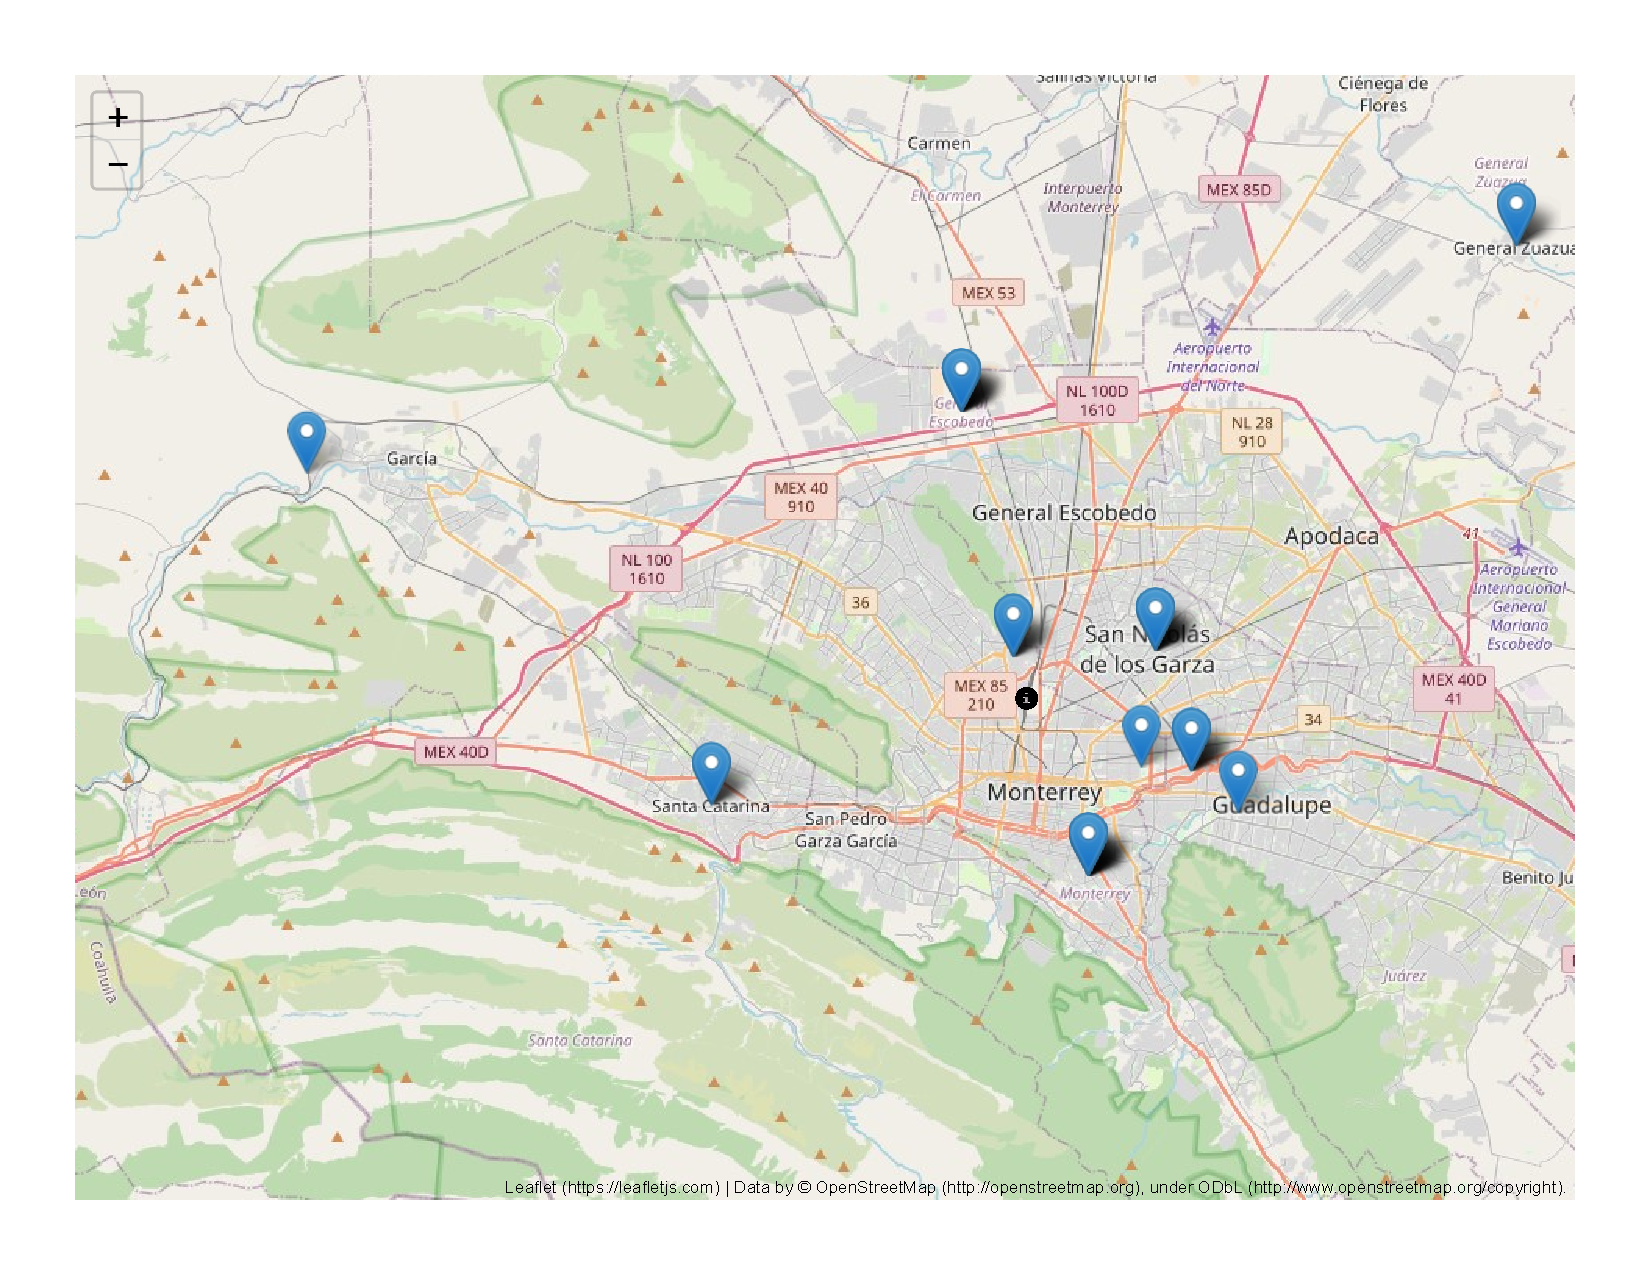
\includegraphics[scale=0.3]{img/deliveries-plot.pdf}
            \caption{Puntos de entrega} 
            \label{puntos-entrega-mapa}
        \end{figure}
    
    \section{Metodología}
    
        Para la solución de esta problemática hemos usado el lenguaje de programación Python; para los procesos de lectura, limpieza, exploración y agregación de datos hemos usado la librería \emph{pandas} en conjunto con \emph{matplotlib} y \emph{seaborn}, para la solución del problema de programación lineal usamos la librería \emph{ortools} de Google, y para la visualización de los rutas generadas hemos usado \emph{folium}. Una liga al código fuente que hemos desarrollado se encuentra en el apéndice \ref{code}.
        
        El dispositivo que usamos para desarrollar y correr la aplicación disponía de un CPU Intel i5 con 8 GB de memoria RAM, como sistema operativo se ha usado Ubuntu 20.04 LTS.
    
        \subsection{Limpieza de la base de datos} \label{stage 1}
            
            Hemos recibido 4 bases de datos. Una conteniendo las direcciones de los centros de distribución de la emppresa en México, un archivo que contiene un listado de todos los productos que vende la empresa más algunas de sus propiedades, en particular nos interesa el volumen de cada artículo. Disponemos también de un archivo que contiene todos los tipos de vehículos que la empresa usa para realizar las entregas, y una base de datos que contiene un listado de las entregas que se deben de realizar.
            
        \subsection{Procesamiento de domicilios} \label{stage 2}
        
            Para la geo-codificación de los domicilios hemos usado la librería \emph{Photon}, desde el paso anterior hemos creado una columna que contiene todos los datos de referencias de los domicilios de los compradores. El proceso de geo-codificación toma un tiempo promedio de 15 minutos en la máquina que usamos, en promedio se logran codificar 25\% de los domicilios que recibe. Al final de este proceso tenemos las coordenadas asociadas a cada uno de los domicilios

        \subsection{Cálculo de matriz de distancias} \label{stage 3}
            
            De las coordenadas de cada domicilio calculamos una matriz de distancia todos contra todos, la distancia a usar es la geodésica.

        \subsection{Generación de rutas} \label{stage 4}
        
            Para la solución del problema hemos usado la librería \emph{ortools} de Google. Hacemos uso de la matriz de distancias calculada en el paso anterior, un listado de cuánto volumen debe de ser entregado a cada uno de los clientes, un número de vehículos a mandar, y su capacidad máxima de carga en metros cúbicos. La solución generada consiste de un listado de las rutas a seguir por cada uno de los vehículos, el volumen total que llevarán, cuál fue la distancia total recorrida por todos los vehículos y cuánta carga llevaron.

        \subsection{Visualización de rutas} 
            
            La visualización de rutas se realizó con la API de la librería \emph{folium}, con ella hemos generado un mapa de Monterrey en la que se visualizan las rutas que siguen todos los vehículos; el mapa también despliega información del domicilio al que se realiza la entrega, y el volumen total de los productos que debe de recibir.
            
    \section{Experimentación y resultados}
    
        La red con la que tratamos consta de 193 nodos, 192 referentes a los clientes, y 1 nodo más para el Centro de Distribución. El número de conexiones (aristas) dentro del grafo es $193\choose2$ = $18528$
    
        Después de correr la aplicación, se desplegará el navegador el conjunto de rutas de todos los vehículos, en la figura \ref{generated-routes} podemos ver 2 de las rutas encontradas.
    
        \begin{figure}[H]
            \centering
            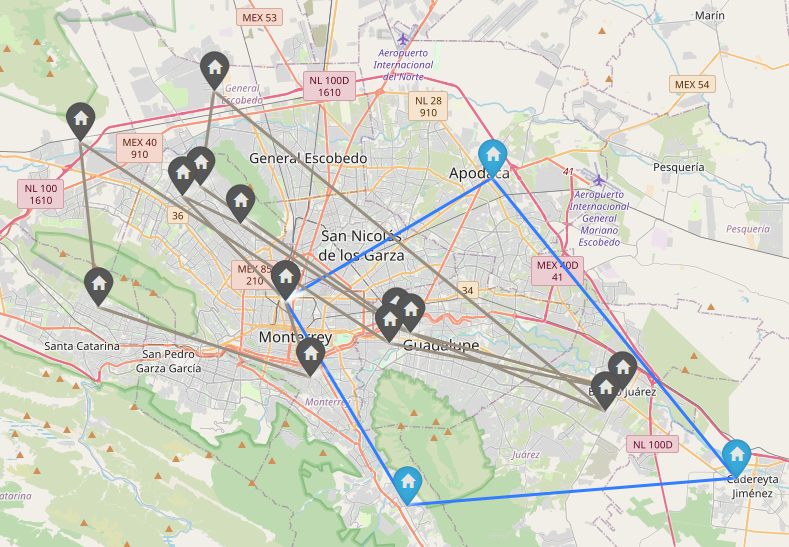
\includegraphics[scale=0.3]{img/rutas-generadas.png}
            \caption{Ejemplo de rutas generadas} 
            \label{generated-routes}
        \end{figure}
        
        Como se puede apreciar en la tabla \ref{rutas}, para esta simulación, la aplicación encontró un conjunto de rutas que minimizan la distancia que recorren los camiones en total hasta 483.49 km. En las mejores corridas la ruta más corta que realiza un camión es de 32 km, y la más larga de 97.02 km.
        
        \begin{table}[h!]
            \centering
            \csvreader[tabular = ||c|c|c|c|c||,
                        table head = \hline N & Distancia $(km)$ & Carga $(m^{3})$ & Vol. muerto $(m^{3})$ & Gas $(l)$ \\ \hline,
                        late after last line = \\ \hline,
                        ]{../data/processed/best_route.csv}{}%
                        {\csvcoli & \csvcolii & \csvcoliii & \csvcoliv & \csvcolv}
            \caption{Rutas generadas por el programa}
            \label{rutas}
        \end{table}
        
    \section{Discusión de resultados} \label{discusion}
        
        A pesar de que el producto que hemos desarrollado ya es funcional, hemos encontrado algunas áreas de oportunidad que de ser resueltas incrementarían aún más el valor de la aplicación:
        
        \subsection{Geo-codificación de los domicilios}
            
            Actualmente la aplicación hace uso de una librería de libre distribución llamada \emph{Photon} para geo-codificar los domicilios disponibles en la base de datos; consideramos que la adquisición de una licencia comercial podría aumentar aún más el número de domicilios que son geo-codificados con éxito.
            
        \subsection{Cálculo de distancia entre 2 puntos}
            
            La aplicación utiliza como métrica de distancia la distancia geodésica, que está relativamente lejos de ser una aproximación rigurosa para determinar la distancia entre 2 puntos. Sugerimos también que se adquiera una licencia comercial que calcule esta distancia. Su uso le daría una mayor validez a los resultados que encontramos.
        
    \section{ODS}
    
        Igual que encontrar la ruta más eficiente para la empresa, buscamos tener un impacto social por esta razón reconocemos la importancia que tiene que la innovación trascienda los objetivos personales, así como a los objetivos colectivos. Por eso mismo, tenemos la intención de tener un impacto positivo en los Objetivos de Desarrollo Sostenible propuestos por la ONU. 
        
        Una de las ODS implementadas en el proyecto es el objetivo número 9,  Industria, Innovación e Infraestructura, ya que los valores de esta ODS se alinean perfectamente con los de nuestro proyecto. Este objetivo tiene como enfoque la construcción de infraestructuras resilientes en forma de rutas adaptables que se basan en las necesidades, la industrialización sostenible en forma de la minimización de kilómetros recorridos y por lo tanto energía ocupada, e innovación de un sistema ya existente. 
        
        Otro de los objetivos en los que impactamos positivamente es el número 11, Ciudades y Comunidades Sustentables, ya que reconocemos que el mundo está cada vez más urbanizado, y la sostenibilidad no se puede quedar atrás. El e-commerce está cada vez más presente en las vidas de la gente, y al minimizar los efectos negativos de esta industria es el mejor paso que podemos tomar para un futuro verde. 

    \section{Conclusiones}    
        
        El ruteo de vehículos sigue siendo uno de los retos más relevantes para la Investigación de Operaciones, el diseño de algoritmos eficientes que logren encontrar rutas de entrega óptimas con cantidades cada vez más grandes de puntos de entrega es un imperativo para cualquier departamento de logística.
        
        Dado el gran número de puntos de entrega y de la enorme cantidad de posibles rutas a explorar, el uso de algoritmos heurísticos que logren encontrar rutas sub-óptimas es una alternativa a considerar para cualquier empresa; el que estos métodos puedan encontrar soluciones buenas en tiempos razonables hace que sean mucho más sencillos de implementar en producción.
        
        El proceso de determinar cuál es el mejor sub-conjunto de rutas tendrá tanto repercusiones económicas para la empresa como ecológicas para el ambiente, el proyecto que hemos desarrollado busca reducir la mayor cantidad de distancia recorrida posible por parte de las rutas, lo cual trae consigo una disminución del gasto realizado en el transporte de sus productos, mientras que se reducen en general las emisiones de carbono de sus vehículos.
        
    \appendices
    
    \section{Código fuente}\label{code}
    
        El código generado puede ser consultado \href{https://github.com/JuanEcheagaray75/capacitated-vrp}{aquí}
    
    \bibliographystyle{IEEEtran}
    \bibliography{references.bib}

\end{document}
